\documentclass[11pt]{article}

\usepackage{xcolor}
\definecolor{darkpastelgreen}{rgb}{0.01, 0.75, 0.24}

\usepackage[colorlinks=true,
            linkcolor=red,
            urlcolor=darkpastelgreen,
            citecolor=blue,
            breaklinks=true]{hyperref}
\usepackage{breakurl} 
\usepackage[a4paper, left=3cm, right=3cm, top=3cm, bottom=3cm]{geometry}
\RequirePackage{amsmath,amsfonts, amssymb,amsthm}

\hypersetup{pdfauthor = {Simon Bussy}}

\usepackage{authblk}
\title{\vspace{-.5cm} Lights: a generalized joint model for high-dimensional multivariate longitudinal data and censored durations \vspace{.5cm}}
\author[1,2]{Simon Bussy\thanks{Corresponding author: \href{mailto:simon.bussy@gmail.com}{\texttt{simon.bussy@gmail.com}}}}
\author[2,3]{Van Tuan Nguyen}
\author[4]{Antoine Barbieri}
\author[1]{Sarah Zohar}
\author[1,5]{Anne-Sophie Jannot}
\affil[1]{INSERM, UMRS 1138, Centre de Recherche des Cordeliers, Paris, France}
\affil[2]{LOPF, Califrais' Machine Learning Lab, Paris, France}
\affil[3]{LPSM, UMR 8001, CNRS, Sorbonne University, Paris, France}
\affil[4]{INSERM, UMR 1219, Bordeaux Population Health Research Center, Univ. Bordeaux, France}
\affil[5]{Biomedical Informatics and Public Health Department, EGPH, APHP, Paris, France}
\setcounter{Maxaffil}{0}
\renewcommand\Affilfont{\itshape\small}

\usepackage{mathtools}
\usepackage{mathrsfs}
\usepackage{mathrsfs} 
\usepackage{natbib}
\usepackage{setspace}
\usepackage{dsfont}
\usepackage{caption}
\usepackage{booktabs}
\usepackage{subfigure}
\usepackage{bm}
\usepackage{tikz}
\usetikzlibrary{fit,shapes,shadows,arrows,positioning,graphs}
\usepackage{algpseudocode}
\usepackage[linesnumbered,ruled,vlined]{algorithm2e}
\newcommand\mycommfont[1]{\footnotesize\ttfamily\textcolor{orange}{#1}}
\SetCommentSty{mycommfont}
\SetKwInput{KwInput}{Input} 
\SetKwInput{KwOutput}{Output}

\newtheorem{assumption}{Assumption}{\bf}{\rm} 
\newtheorem{lemma}{Lemma}

\DeclareMathOperator{\argmin}{argmin}
\DeclareMathOperator{\Tr}{Tr}

\newcommand{\dd}{\mathrm{d}}
\newcommand{\ind}[1]{\mathds{1}_{#1}}
\newcommand{\norm}[1]{\|#1\|}
\newcommand{\cY}{\mathcal Y}
\newcommand{\cD}{\mathcal D}
\newcommand{\cC}{\mathcal C}
\newcommand{\cG}{\mathcal G}
\newcommand{\cN}{\mathcal N}
\newcommand{\cA}{\mathcal A}
\newcommand{\cQ}{\mathcal Q}
\newcommand{\cU}{\mathcal U}
\newcommand{\cR}{\mathcal R}
\newcommand{\cH}{\mathcal H}
\newcommand{\cB}{\mathcal B}
\newcommand{\cS}{\mathcal S}
\newcommand{\cI}{\mathcal I}
\newcommand{\R}{\mathds R}
\newcommand{\N}{\mathds N}
\newcommand{\E}{\mathds E}
\renewcommand{\P}{\mathds P}
\newcommand{\bSigma}{\textbf{$\Sigma$}}

\date{}

\begin{document}

\maketitle

\vspace{-.5cm}
\begin{abstract}

This paper introduces a prognostic method called \textit{lights} to deal with the problem of joint modeling of longitudinal data and censored durations, where a large number of both longitudinal and time-independent features are available. 
In the literature, standard joint models are either of type shared random-effect or joint latent class ones ; where the association structure between the longitudinal and the time-to-event submodels takes respectively the form of either shared association features learned from the longitudinal processes and included as potential risk factor in the survival model, or latent classes modeling population heterogeneity.
We pick modeling ideas from both worlds and use appropriate penalties during inference for being able to learn from a high-dimensional context.
The statistical performance of the method is examined on an extensive Monte Carlo simulation study, and finally illustrated on a publicly available dataset.
Our proposed method significantly outperforms the state-of-the-art joint models regarding risk prediction in terms of C-index in a so-called real-time prediction paradigm, with a computing time orders of magnitude faster. In addition, it provides powerful interpretability by automatically pinpointing significant features being relevant from a practical perspective. Thus, we propose a powerfull tool with the ability of automatically determining significant prognostic longitudinal features, which is of increasing importance in many areas: for instance personalized medicine, or churn prediction in a customer profile and activity monitoring setting, to name but a few.\\
\noindent
\emph{Keywords.} High-dimensional estimation; Joint modeling; Multivariate longitudinal data; Survival analysis
\end{abstract}

\section{Introduction}

\paragraph{General framework.}

<<<<<<< HEAD
With classical setting of survival analysis where we denote $T^\star$ and $C$ are the times of the event of interest and censoring times respectively.
We then denote $T$ the right-censored time and $\Delta$ the censoring indicator, defined as 
\begin{equation*}
T = T^\star \wedge C \quad \text{and} \quad \Delta = \ind{\{T^\star \leq C\}}
\end{equation*}
=======
The setting of this paper is such that we want to incorporate high-dimensional time-dependent (longitudinal) features measured with error in a survival model. Let us consider the usual survival analysis framework.
Following~\citet{andersen2012statistical}, let non-negative random variables $T^\star$ and $C$ stand for the times of the event of interest and censoring times respectively.
We then denote $T$ the right-censored time and $\Delta$ the censoring indicator, defined as $T = T^\star \wedge C \quad \text{and} \quad \Delta = \ind{\{T^\star \leq C\}}$
>>>>>>> e1bafc1e34a8c64e9c698da90b09546387e3caf4
respectively, where $a \wedge b$ denotes the minimum between two numbers $a$ and $b$, and $\ind{\{\cdot\}}$ the indicator function taking the value $1$ if the condition in $\{\cdot\}$ is satisfied and $0$ otherwise.

Let $X$ denotes the $p$-dimensional vector of time-independent features and let  $Y(t) = \big(Y^1(t), \ldots, Y^L(t) \big)^\top \in \R^L$ denote the value of the $L$-dimensional longitudinal outcome at time point $t \geq 0$, with $L \in \N_+$.

\paragraph{Heterogeneity of the population.}

Assume the population that can be devided into a finite number K of latent homogeneous subgroups. Let us denote $\pi_{\xi_k}(x) = \P[G=k|X=x]$ the latent class membership probability given time-independent features $x \in \R^p$, and consider a softmax link function given by $\pi_{\xi_k}(x) = e^{x^\top\xi_k} / \sum_{k=0}^{K-1}e^{x^\top\xi_k}$
where $\xi_k \in \R^p$ denotes a vector of time-independent parameters.

\section{Method}
\label{sec:Method}

In this section, we descibe the longitudinal and time-to-event submodels, as well as the required hypothesis in order to write a likelihood and draw inference for the lights model.

\subsection{Class-specific marker trajectories}

We suppose a class-specific marker trajectory and a generalized linear mixed model for each longitudinal marker given latent class $G$, so that for the $l$-th outcome at time $t \geq 0$ one has $h_l\big(\E[Y^l(t)|b^l, G=k]\big) = m_k^l(t)$ where $h_l$ denotes a known one-to-one link function, and $m_k^l$ the linear predictor such that $m_k^l(t) = u^l(t)^\top\beta_k^l + v^l(t)^\top b^l$ where $u^l(t) \in \R^{q_l}$  and $v^l(t) \in \R^{r_l}$ are row vectors of (possibly) time-varying features  with $r_l \leq q_l$.
The random effects component is assumed to be followed a zero-mean multivariate normal distribution~\citep{hickey2016joint}, that is $b^l \sim \cN(0, D_{ll})$
with $D_{ll} \in \R^{r_l \times r_l}$ the unstructured variance-covariance matrix. And we denote $D$ the global variance-covariance matrix.

In the sequel of the paper, our aim is to associate the true and unobserved value $m_k^l(t)$ of the $l$-th longitudinal outcome at time $t$ with the event outcome $T^\star$.

\subsection{Class-specific risk of event}

To quantify the effect of the longitudinal outcomes on the risk for an event, we use a Cox~\citep{Cox1972JRSS} relative risk model of the form
\begin{equation*}
  \label{eq:intensity-model}
  \lambda(t|\cY(t), G = k) = \lambda_0(t) \exp \Big\{\sum_{l=1}^L \sum_{a=1}^\cA {\gamma_{k,a}^l} \Psi_a^l(t) \Big\},
\end{equation*}
where $\lambda_0(\cdot)$ is an unspecified baseline hazard function and given that $G = k$, we denote $\cY^l(t) = \{Y^l(u), 0 \leq u < t\}$ and $\cY(t) = \bigcup_{l=1}^L \cY^l(t)$ the history of the true longitudinal process up to time $t$.
For each $l$-th longitudinal outcome, we consider $\cA \in \N_+$ known functionals $\Psi_a^l$ extracted from $\cY^l(t)$ through a given representation mapping, and $\gamma_{k,a}^l \in \R$ the corresponding joint representation parameters.  

Let us finally denote $\gamma_k= (\gamma_{k,1}^1, \ldots, \gamma_{k,\cA}^1, \ldots, \gamma_{k,1}^L, \ldots, \gamma_{k,\cA}^L )^\top \in \R^{L\cA}$, so that one has $\lambda(t|\cY(t), G = k) = \lambda_0(t) \exp \big\{\gamma_k^\top \Psi(t) \big\}$, where $\Psi(t) \in \R^{L\cA}$ denotes the representation features vector.

\subsection{Generalization of SREMs and JLCMs}
 
Our model is clearly of JLCMs type, and can be viewed as a generalization of SREMs type in a much more flexible way. Our proposition differs from standard SREMs in two respects: $(i)$ representation vector $\Psi(t)$ does not depend on the modeling assumptions in the longitudinal submodel and $(ii)$ it allows to choose multiple high-dimensional representation mappings that characterize time series and concatenate them, since we perform features selection through the regularization strategy described in Section~\ref{sec:penalized-obj}. Point $(i)$ is key since for instance the $\beta_k^l$ dependence in $\Psi_a^l$ would lead to complicated updates, while the $b^l$ dependence would lead to untracktable integrals that are common in SREMs and require approximation methods such as Monte Carlo~\citep{hickey2018joinerml}, being computationally intensive and not scalable in a high-dimensional context. For point $(ii)$ in practice, we use the \texttt{Python} library \texttt{tsfresh}~\citep{christ2018time} and include many extracted features, such as absolute energy of the time series, statistics on autocorrelation, or Fourier and wavelet basis projections, to name but a few.

\subsection{Likelihood}

Consider an independent and identically distributed (i.i.d.) cohort of $n$ subjects
\[ \cD_n = \big\{ (x_1, y_1^1, \ldots, y_1^L, t_1, \delta_1), \ldots, (x_n, y_n^1, \ldots, y_n^L, t_n, \delta_n) \big\} \]
where $y_i^l=(y_{i1}^l, \ldots, y_{in_i^l}^l)^\top \in \R^{n_i^l}$ with $y_{ij}^l=Y_i^l(t_{ij}^l)$ for all $l=1, \ldots, L$. 
For the $i$-th subject, let us denote $y_i = ({y_i^1}^\top \cdots {y_i^L}^\top)^\top \in \R^{n_i}$ and $b_i = ({b_i^1}^\top \cdots {b_i^L}^\top)^\top \in \R^r$, with $n_i = \sum_{l=1}^L n_i^l$ and $r = \sum_{l=1}^L r_l$ the total number of longitudinal measurements (for subject $i$) and the total dimension of the random effects respectively, as well as the following design matrices
\[ U_i = 
\begin{bmatrix}
  U_{i1} & \cdots & 0\\
  \vdots &  \ddots & \vdots \\
  0 & \cdots & U_{iL}
\end{bmatrix} 
\in \R^{n_i \times q}
\qquad \text{and} \qquad
V_i = 
\begin{bmatrix}
  V_{i1} & \cdots & 0\\
  \vdots &  \ddots & \vdots \\
  0 & \cdots & V_{iL}
\end{bmatrix}
\in \R^{n_i \times r}
\]
with $q = \sum_{l=1}^L q_l$ and where for all $l=1, \ldots, L$, one writes $U_{il} = \big(u_i^l(t_{i1}^l)^\top \cdots u_i^l(t_{in_i^l}^l)^\top\big)^\top \in \R^{n_i^l \times q_l}$ and $V_{il} = \big(v_i^l(t_{i1}^l)^\top \cdots v_i^l(t_{in_i^l}^l)^\top\big)^\top \in \R^{n_i^l \times r_l}$.
We also denote $\beta_k = ({\beta_k^1}^\top \cdots {\beta_k^L}^\top)^\top \in \R^q$ the fixed effect parameter of linear mixed effect model of group $k$ and $M_{ik} = U_i\beta_k + V_ib_i \in \R^{n_i}$ the linear predictor vector for subject $i$ given the fact that he belongs to group $k$.
For the collection of the $\vartheta \in \N_+$ unknown parameters to estimate, we denote 
\[ \theta = \big(\xi_0^\top \cdots \xi_{K-1}^\top, \beta_0^\top \cdots \beta_{K-1}^\top, \phi^\top, \text{vech}(D), \lambda_0^\top, \gamma_0^\top \cdots \gamma_{K-1}^\top\big)^\top \in \R^\vartheta .\]

The conditional distribution of $y_i|b_i, G_i=k$ is then assumed to be from a distribution with a density of the form $f(y_i|b_i, G_i=k) = \exp \big\{(y_i \odot \Phi_i)^\top M_{ik} - c_\phi(M_{ik}) + d_\phi(y_i) \big\}$,
with $\Phi_i = (\phi_1^{-1} {\textbf{1}_{n_i^1}}^\top \cdots \phi_L^{-1} {\textbf{1}_{n_i^L}}^\top)^\top \in \R^{n_i}$ and $\phi = (\phi_1, \ldots, \phi_L)^\top \in \R^L$.
The likelihood of survival model can be written as
\[f_\theta(t_i, \delta_i| G_i = k) = \big[\lambda(t_i|\cY_i(t_i), G_i = k)\big]^{\delta_i} \exp \Big\{-\int_0^{t_i} \lambda(s|\cY_i(s), G_i = k) \dd s \Big\}. \]
Then, the log-likelihood of joint model in type of JLCMs based on these 2 above likelihoods is given by
\begin{equation*}
    \ell_n(\theta) = \ell_n(\theta ; \cD_n) = n^{-1} \sum_{i=1}^n \log \sum_{k=0}^{K-1} \pi_{\xi_k}(x_i) f_\theta(t_i, \delta_i| G_i = k) f_\theta(y_i | G_i = k),
\end{equation*}
\
\section{Inference}
\label{sec:inference}

\subsection{Penalized objective}
\label{sec:penalized-obj}

In order to avoid overfitting and improve the prediction power of our method, we propose to minimize the penalized objective
\begin{equation*}
    \ell_n^\text{pen}(\theta) = - \ell_n(\theta) + \sum_{k=0}^{K-1} \zeta_{1,k} \norm{\xi_k}_{\text{en}, \eta} + \zeta_{2,k} \norm{\gamma_k}_{\text{sg} l_1, \tilde{\eta}}
\end{equation*}
with the elastic net penalty $\norm{z}_{\text{en}, \eta} = (1-\eta)\norm{z}_1 + \dfrac\eta2 \norm{z}_2^2$ and the sparse group lasso penalty $\norm{z}_{\text{sg} l_1, \tilde{\eta}} = (1-\tilde{\eta})\norm{z}_1 + \tilde{\eta} \sum_{l=1}^L\norm{z}_{2,l}$.
Hence, the resulting optimization problem is written $\hat \theta \in \argmin_{\theta \in \R^\vartheta} \ell_n^\text{pen}(\theta).$

\subsection{A Proximal Quasi-Newton EM}
\label{sec:prox-QNEM}

In order to derive an algorithm for this objective, we introduce a so-called prox-QNEM algorithm. We first need to compute the negative completed log-likelihood by
\begin{align*}
  \ell_n^\text{comp}(\theta) &= \ell_n^\text{comp}(\theta ; \cD_n, \textbf{\textit{b}}, \textbf{\textit{G}}) = - n^{-1} \sum_{i=1}^n -\dfrac12 (r \log 2\pi + \log|D| + b_i^\top D^{-1}b_i) \\ 
  &+ \sum_{k=0}^{K-1} \ind{\{G_i=k\}} \Big[ \log \pi_{\xi_k}(x_i) + \delta_i \Big(\log \lambda_0(t_i) + \gamma_k^\top \Psi_i(t_i) \Big) \\ 
  &- \int_0^{t_i} \lambda_0(s) \exp \big\{ \gamma_k^\top \Psi_i(s) \big\} \dd s  + (y_i \odot \Phi_i)^\top M_{ik} - c_\phi(M_{ik}) + d_\phi(y_i) \Big].
\end{align*}
Suppose that we are at step $w + 1$ of the algorithm, with current iterate denoted $\theta^{(w)}$. 

\paragraph*{E-step.}

We need to compute the expected negative log-likelihood of the complete data conditional on the observed data and the current estimate of the parameters given by $\cQ_n(\theta, \theta^{(w)}) = \E_{\theta^{(w)}}[\ell_n^\text{comp}(\theta) | \cD_n]$.
Then, the previous expression requires to compute expectations of the form
\[ \E_{\theta^{(w)}}[ g(b_i, G_i) | t_i, \delta_i, y_i] = \sum_{k=0}^{K-1} \pi_{ik}^{\theta^{(w)}} \int_{\R^r} g(b_i, G_i) f(b_i | t_i, \delta_i, y_i ; \theta^{(w)}) \dd b_i \]
for different functions $g$, where we denote $\pi_{ik}^{\theta^{(w)}} = \P_{\theta^{(w)}}[G_i = k | t_i, \delta_i, y_i]$ the posterior probability of the latent class membership using parameters $\theta^{(w)}$.

\paragraph*{Proximal Quasi-Newton M-step.}
Here, we need to compute \[\theta^{(w+1)} \in \argmin_{\theta \in \R^\vartheta} \cQ_n(\theta, \theta^{(w)}) + \sum_{k=0}^{K-1} \zeta_{1,k} \norm{\xi_k}_{\text{en}, \eta} + \zeta_{2,k} \norm{\gamma_k}_{\text{sg} l_1, \tilde{\eta}}.\]
First, the update of $D^{(w)}$ is given in closed-form by $D^{(w+1)} = n^{-1} \sum_{i=1}^n \E_{\theta^{(w)}}[ b_i b_i^\top | t_i, \delta_i, y_i]$.
Then, let us focus on the update of $\xi_k^{(w)}$ for $k=0, \ldots, K-1$. We denote $P^{(w)}_{n, k}(\xi_k) = -n^{-1} \sum_{i=1}^n \sum_{k=0}^{K-1} \pi_{ik}^{\theta^{(w)}} \log \pi_{\xi_k}(x_i)$ based on the quantities involved in $\cQ_n(\theta, \theta^{(w)})$ that depend on $\xi_k$. The update for $\xi_k^{(w)}$ therefore requires to solve the following convex minimization problem
\begin{equation*}
  \xi_k^{(w+1)} \in \argmin_{\xi_k \in \R^p} P^{(w)}_{n,k}(\xi_k) + \zeta_{1,k} \norm{\xi_k}_{\text{en}, \eta}.
\end{equation*}
We then choose to solve using the L-BFGS-B algorithm  which belongs to the class of quasi-Newton optimization routines.
The update of $\beta_k^{(w)}$ for $k=0, \ldots, K-1$ is obtained in closed-form. Then, we use proximal gradient (ISTA) for the $\gamma_k^{(w+1)}$ update, based on Lemma 1 that states $\text{prox}_{\text{sg} l_1,\tilde \eta, \zeta} = \text{prox}_{\zeta \tilde \eta \sum_{l=1}^L \norm{\cdot}_{2,l}} \circ \text{prox}_{\zeta (1 - \tilde \eta) \norm{\cdot}_1}$. 
The closed-form update of $\lambda_0^{(w)}$ is given by
\begin{equation*}
  \lambda_0^{(w+1)}(t)= \dfrac{\sum_{i=1}^n \delta_i \ind{\{t=t_i\}}}{\sum_{i=1}^n \sum_{k=0}^{K-1} \pi_{ik}^{\theta^{(w)}} \exp \big\{{\gamma_k^{(w+1)}}^\top \Psi_i(t)\big\} \ind{\{t_i \geq t\}} },
\end{equation*}
for all $t \geq 0$, which is a Breslow like estimator~\citep{breslow1972contribution} adapted to our model. 

\noindent Finally, the update of $\phi^{(w)}$ is obtained in closed-form.
\begin{align*}
  \phi_l^{(w+1)} = \big(\sum_{i=1}^n n_i^l \big)^{-1} &\sum_{i=1}^n \sum_{k=0}^{K-1} \pi_{ik}^{\theta^{(w)}} \Big[ \big(y_i^l - U_{il} {\beta_k^l}^{(w+1)}\big)^\top \Big(y_i^l - U_{il} {\beta_k^l}^{(w+1)} \nonumber \\
  & - 2V_{il} \E_{\theta^{(w)}}[ b_i^l | t_i, \delta_i, y_i]\Big) + \Tr\big(V_{il}^\top V_{il} \E_{\theta^{(w)}}[ b_i^l {b_i^l}^\top | t_i, \delta_i, y_i]\big) \Big].
\end{align*}

\section{Performance evaluation}

\paragraph{Real-time prediction paradigm.}

Once the learning phase is achieved for the model on a training set (so that  $\hat\theta$ is obtained, we want to assess real-time risk prediction performances on a test set. Denoting $t^{max}_i$ the time for subject $i$ when one wants to perform the risk prediction -- so in practice, the time up to which one has data measurements for $Y_i$, say the ``present'' time for prediction.

\paragraph{Predictive marker.}
Posterior risk classification for subject $i$ and latent class $k$ is chosen to be marker rule of the lights 
\begin{equation}
  \label{eq:marker-def}
  \P_{\hat \theta}[G_i=k | T_i > t^{max}_i, \tilde y_i] = \dfrac{\pi_{\hat \xi_k}(x_i) f_{\hat \theta}(t^{max}_i, \delta_i=0, \tilde y_i | G_i=k)}{\sum_{k=0}^{K-1} \pi_{\hat \xi_k}(x_i) f_{\hat \theta}(t^{max}_i, \delta_i=0, \tilde y_i | G_i=k)}
\end{equation}

\subsection{The C-index metric}
\label{sec:Metrics}
We use concordance index (C-index) to evaluate risk prediction performances
\begin{equation*}
  \cC_\tau =\P[\hat \cR_i > \hat \cR_j | T_i < T_j , T_i < \tau],
\end{equation*}
with $\tau$ corresponding to the fixed and prespecified follow-up period duration \citep{heagerty2005survival}.

\subsection{Simulation}
The below figures are obtained on simulated data with 2 latent groups. They are  learning curve over time of log-likelihood function, estimation of parameters compare to the true ones.
\begin{figure}[!ht]
\centering
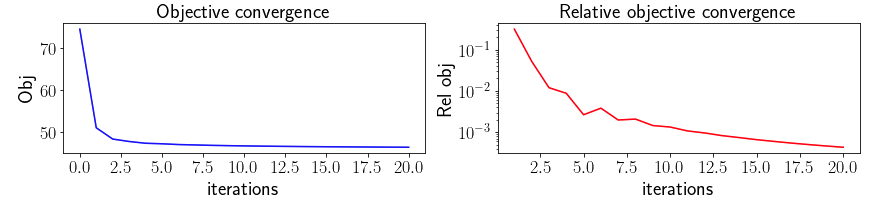
\includegraphics[width=.85\textwidth]{./figures/obj_vcg}
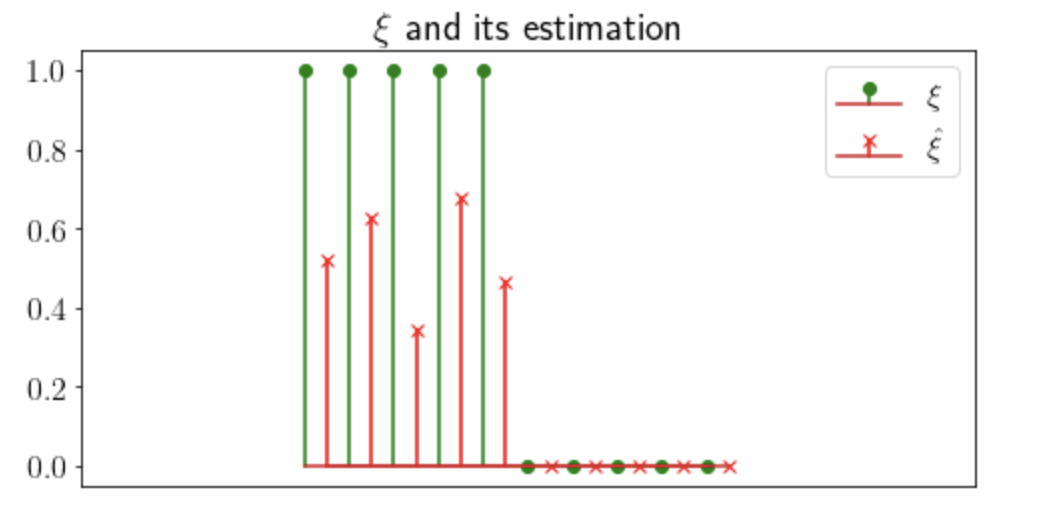
\includegraphics[width=.37\textwidth]{./figures/xi_estimation}
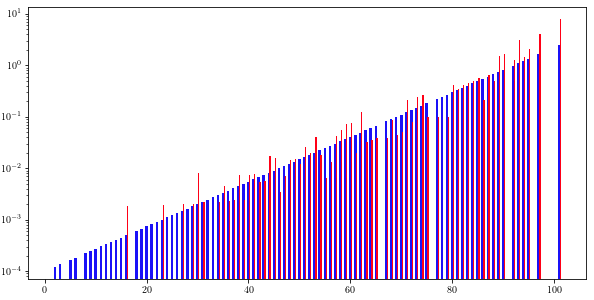
\includegraphics[width=.37\textwidth]{./figures/baseline_estimation}
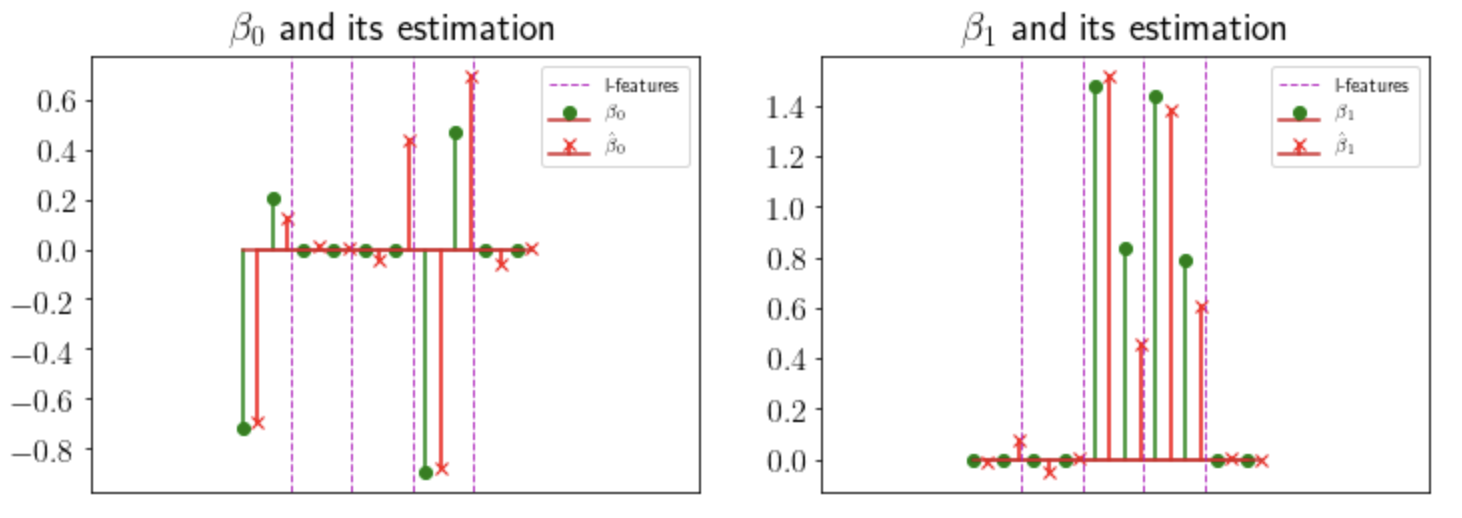
\includegraphics[width=.8\textwidth]{./figures/beta_estimation}
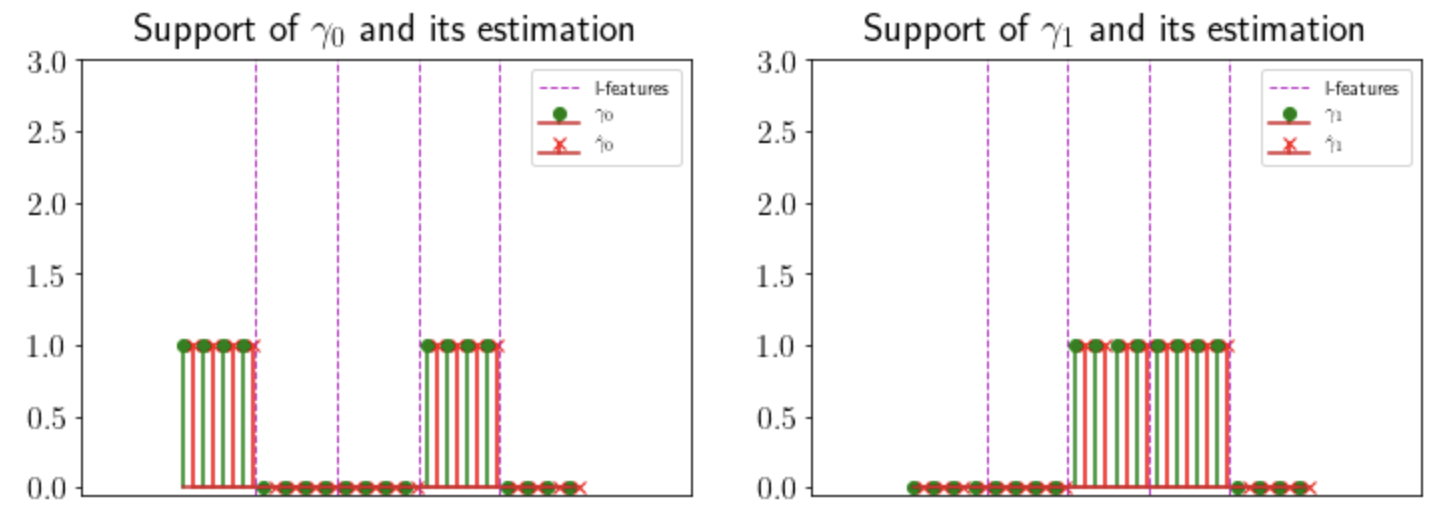
\includegraphics[width=.8\textwidth]{./figures/gamma_estimation}
\end{figure}

\footnotesize
\bibliography{biblio}
\bibliographystyle{plainnat}{}
\end{document}
